\documentclass[conference]{IEEEtran}
\usepackage{amsmath,amssymb}
\usepackage{newtxtext,newtxmath}
\usepackage{graphicx,booktabs,url}
\usepackage[hidelinks]{hyperref}
% Generated from audited measured experiment artifacts.
\newcommand{\BaselineAbstract}{Fresh predictions match all six author-stored language/configuration outputs exactly, and an independent scorer agrees with the original metric scripts.}

\newcommand{\ExtensionAbstract}{On 40 reserved Chef files with 16 annotated administrative-default occurrences, recall increases from 43.75\% to 68.75\%, precision from 87.50\% to 91.67\%, and F1 from 58.33\% to 78.57\%. The extension recovers 4 missed occurrences without adding false positives; Ansible and Puppet oracle results remain unchanged.}

\newcommand{\PartitionDescription}{Development comprises 40 files per technology (120 total); test comprises 41 Ansible, 40 Chef, and 40 Puppet files (121 total). Entire files, including all their labels, remain in one partition. File hashes and membership are recorded; related originating projects are not guaranteed disjoint.}

\newcommand{\DevelopmentEvidence}{In Chef development files, the reproduced administrative-default detector has TP=8, FP=0, and FN=13. Manual inspection of development false negatives identifies literal MySQL users in command guards, heredoc shell scripts, a status-command assignment, and an opaque Ruby block. Other missed annotations refer to unresolved database-user attributes rather than an explicit literal root option. The proposed rule recovers 8 development occurrences without new false positives; it deliberately leaves runtime-variable cases unresolved.}

\newcommand{\RuleDescription}{The rule processes command-related IR variable/attribute fields and their source slices. Supported roles include command, cmd, shell, execute, code, block, only\_if, not\_if, and identifiers ending in \_cmd or \_command. In opaque command blocks it recognizes explicit Ruby system/exec/spawn or shell-literal wrappers. A source assignment can also recover a literal command whose IR value was replaced by an interpolation function node. Shell-like tokens distinguish supported executables (mysql, mysqladmin, mysqldump, mysqlcheck) from quoted mentions. A report requires a literal root user given by -uroot, -u root, --user=root, or --user root before the SQL execution payload. Leading environment assignments and command chaining are supported. Unresolved user expressions, root-like substrings, arbitrary wrappers, and option-file defaults are not inferred. The same implementation applies to all three technologies; no benchmark filenames or oracle labels are used in recognition.}

\newcommand{\ReproductionDiscussion}{All six native prediction multisets match the author outputs: improved and SLIC/SLAC-like configurations for each language. Ansible equality is checked over file/category/content because the stored output lacks line numbers; Chef and Puppet equality uses file/line/category. The independently implemented scorer agrees with all six original scorer runs. Per-category counts are identical. Puppet macro precision is 0.686 before rounding, displayed as 0.69, versus the paper's 0.68; averaging the paper's already-rounded per-category precisions gives 0.684, displayed as 0.68. This is an aggregation-rounding difference, not a prediction gap. Four Ansible file types yield no IR in the original parser; these are retained in the evaluated population and their diagnostics are disclosed, not silently dropped or described as successfully parsed.}

\newcommand{\BaselineTable}{\begin{table}[t]\centering\caption{Published and reproduced improved-GLITCH averages.}\label{tab:baseline}
\begin{tabular}{lrrrr}\toprule
Technology & Paper P & Paper R & Native P & Native R \\\midrule
Ansible & 0.77 & 0.87 & 0.77 & 0.87 \\
Chef & 0.77 & 0.86 & 0.77 & 0.86 \\
Puppet & 0.68 & 0.85 & 0.69 & 0.85 \\
\bottomrule\end{tabular}\par\smallskip\emph{Native averages use unrounded category values, include the separate No smell class and exclude undefined values. Puppet's one-hundredth precision difference is explained by averaging rounded cells; prediction multisets and counts match exactly.}\end{table}}

\newcommand{\ExtensionDiscussion}{The primary reserved-test comparison is Chef administrative-default detection: TP/FP/FN changes from 7/1/9 to 11/1/5. Recall improves by 25.00 percentage points and F1 by 20.24 percentage points, with no added false positives. Administrative-default results on reserved Ansible and Puppet files remain unchanged; parser integration tests establish cross-language behavior on controlled examples, not additional real-world gains. The eight unrelated security-smell categories remain unchanged because the visitor only adds administrative-default reports. The paper's separate No smell file-level class may change as additional smells are detected.}

\newcommand{\ExtensionTable}{\begin{table}[t]\centering\caption{Reserved Chef administrative-default results (40 files).}\label{tab:extension}
\begin{tabular}{lrrrrrr}\toprule
Method & TP & FP & FN & P & R & F1 \\\midrule
Archived GLITCH & 7 & 1 & 9 & 0.875 & 0.438 & 0.583 \\
Command-aware & 11 & 1 & 5 & 0.917 & 0.688 & 0.786 \\
Naive substrings & 15 & 10 & 1 & 0.600 & 0.938 & 0.732 \\
\bottomrule\end{tabular}\par\smallskip\emph{Point estimates on 16 annotated occurrences. Rule and ablation were frozen before test scoring. These are smell detections, not confirmed vulnerabilities.}\end{table}}

\newcommand{\AblationDiscussion}{The deliberately weak substring ablation adds a report when an IR source line contains both mysql and root. It attains test recall 0.938 but incurs 10 false positives, compared with 1 for the command-aware rule. Its F1 is 0.732, below the command-aware value 0.786. The ablation is a frozen mechanistic control, not a claimed competitive analyzer. On the full 80-file Chef oracle, the command-aware result is TP=27, FP=1, FN=10 (precision 0.964, recall 0.730, F1 0.831); these full-oracle numbers include development files and are descriptive rather than held-out validation.}

\newcommand{\VerificationDiscussion}{All 15 audit checks pass. The original source remains unchanged, partition/source hashes match, the rule freeze is intact, all original reports are preserved, and only the target smell receives new reports. Independent scores agree with nine original scorer runs covering baseline, command-aware, and naive methods across languages. Three representative files are reparsed and replayed successfully. There are 35 automated correctness and integration tests. The frozen rule timestamp is 2026-11-16; no post-test rule edits are made. Native execution uses Python 3.10.15 and Ruby 2.6.10 on arm64 macOS. Summed per-file times for the improved original and command-aware runs over 241 files are 23.37 and 10.63 seconds, respectively. These single-run timings include parsing, exclude download/setup, and do not establish a statistically reliable speed difference.}

\newcommand{\SpecificLimitations}{The original Chef oracle contains duplicated labels at the same file/line/category; we retain these for faithful reproduction instead of repairing ground truth. Unresolved database-user variables and unsupported command constructs remain false negatives. The rule stops before the SQL execution payload, so it does not resolve user overrides after that payload or full shell/Ruby semantics. Reported gains apply to the archived analyzer and this oracle; they are not proof of generalization to current GLITCH releases or modern production repositories.}

\newcommand{\MeasuredConclusion}{We reproduce the archived GLITCH accuracy evaluation exactly at the stored-prediction level and verify its matching protocol independently. A development-motivated, frozen command-aware extension improves reserved Chef administrative-default F1 from 0.583 to 0.786, recovering 4 missed occurrences without additional false positives. The correction does not improve every smell or every language; Ansible and Puppet oracle scores remain unchanged. The measured outcome supports a bounded implementation contribution with explicitly limited generalization.}

\title{Command-Aware Administrative-User Detection in Infrastructure as Code: An Artifact-Based Extension of GLITCH}
\author{\IEEEauthorblockN{Simone Rodrigues}
\IEEEauthorblockA{IIIT Dharwad\\Dharwad, India\\simonerodrigues12159@gmail.com}}
\begin{document}
\maketitle
\begin{abstract}
Infrastructure-as-Code analyzers must identify security smells across heterogeneous configuration languages. We reproduce the labeled accuracy evaluation of GLITCH, an ASE 2022 technology-agnostic analyzer, using its original archived source, parser dependency, configurations, annotations, and oracle scripts. Rather than applying a new tool version to a different dataset, we compare freshly generated predictions with author-stored results and independently verify the original matching protocol. \BaselineAbstract{}
Motivated by observed development errors and the paper's discussion, we extend administrative-user detection to literal database users embedded in command-valued intermediate-representation nodes. A lexical recognizer distinguishes executable database commands from quoted mentions and unresolved user expressions, without executing infrastructure scripts. The rule is frozen before evaluating reserved file-disjoint test data. \ExtensionAbstract{}
The contribution is a bounded, reproducible correction to the archived analyzer, not proof that every administrative command is exploitable or that a small oracle represents production clouds.
\end{abstract}
\begin{IEEEkeywords}
cloud security, Infrastructure as Code, static analysis, security smells, reproducibility, least privilege
\end{IEEEkeywords}

\section{Introduction}
Infrastructure as Code (IaC) enables repeatable configuration of cloud servers, services, and application environments. Configuration mistakes can nevertheless embed weak credentials, excessive privileges, or insecure communication patterns. GLITCH~\cite{glitch2022} translates Ansible, Chef, and Puppet scripts into a common intermediate representation (IR), enabling reusable detection rules instead of separate language-specific implementations.

A meaningful extension requires both a trustworthy baseline and an observed limitation. We therefore select the base study by artifact availability: its archived package~\cite{artifact} includes original source, parser dependency, manually annotated oracles, and stored outputs. The objective is not to optimize arbitrary results until they resemble published tables. It is to establish reproduction fidelity, identify a development-set failure mechanism, and evaluate one narrowly defined correction on reserved files.

We address three questions: RQ1, can the archived accuracy evaluation be reproduced natively; RQ2, which baseline failure mechanism motivates the extension; and RQ3, does the frozen correction improve administrative-user detection without altering unrelated smells? Contributions are an independently audited oracle reproduction, a reusable command-aware IR rule, and measured development/test results with negative and boundary-case tests. We do not claim the first-ever command analyzer or comprehensive least-privilege verification.

\section{Background and Related Work}
SLIC~\cite{slic} identified security smells in Puppet; SLAC~\cite{slac} extended this line of research to Ansible and Chef. Their language-specific implementations motivate GLITCH's common IR~\cite{glitch2022}. Unit blocks contain variables, attributes, atomic units, conditions, and comments; each retains source locations and, where applicable, information about variable references. The original detector applies configurable name/value patterns to these elements.

GLITCH's nine security smells include administrative defaults, empty passwords, hard-coded secrets, invalid IP binding, suspicious comments, HTTP without TLS, missing integrity checks, weak cryptography, and missing default case branches. A smell indicates a potentially problematic coding pattern, not a confirmed exploit. The administrative-default category relates to unnecessary privileges, CWE-250~\cite{cwe250}.

The base paper reports Chef administrative-default recall of 0.41 and explicitly discusses root users embedded in commands such as \texttt{mysql -uroot}. Its rule examines user-named fields and can miss a literal user encoded in a command-valued field. The MySQL command interface exposes the user through short and long options~\cite{mysql}. Shell-like lexical analysis~\cite{shlex} offers a lightweight way to recognize these options while avoiding unrestricted substring matching. Our contribution extends this archived rule on common IR elements; claims of novelty beyond this baseline require a broader literature and current-tool review.

\section{Artifacts and Reproduction Protocol}
\subsection{Version and Provenance}
We use version 2 of the authors' archived replication package~\cite{artifact}, not GLITCH's current development branch or the separate Zenodo v1.0.0 source release. The original GLITCH source version, configurations, and \texttt{puppetparser 0.1.3} dependency are preserved. Source checksums and revision information are provided in the public repository to support reproducibility.

The package contains the original 81 Ansible, 80 Chef, and 80 Puppet oracle scripts and majority-vote annotations. We analyze all 241 scripts with original improved and SLIC/SLAC-like configurations. Individual file enumeration ensures coverage, while original parsers and visitors remain unchanged. Chef scripts remain in the artifact's \texttt{recipes} folder; no configuration scripts are executed. Ruby Ripper parses source rather than evaluating recipes.

\subsection{Original Matching and Sensitivity}
Fresh predictions are distinguished from author-cached outputs. We independently implement the original technology-specific scoring and run the authors' unmodified scorer scripts on native predictions. Chef and Puppet primarily match file, line, and category, with category-specific file-level exceptions. Ansible's original output lacks line numbers: it matches reported key/value or comment content against the annotated source line. Native exact-line sensitivity is reported separately. We do not silently replace these matching protocols with a different metric while calling the result a reproduction.

Hard-coded password and user reports are subtypes, not additional categories in the nine-smell scores. The paper's ``No smell'' category is a separate file-level class. Undefined precision/recall is not converted into evidence of perfect performance. We retain raw predictions, parse diagnostics, per-category counts, package versions, and hashes.

\subsection{Scope and Partition}
The scope is the labeled accuracy experiment, not the unlabelled frequency study over 196,755 scripts. The latter is much larger; the authors report approximately 1,400 minutes for Chef analysis alone. Full-corpus density and timing results are not claimed here.

Before inspecting individual baseline errors or implementing the extension, files are ordered by a fixed SHA-256 key and partitioned approximately 50/50 into development and reserved test sets within each technology. \PartitionDescription{}
Baseline reproduction uses the complete oracle, whereas extension design uses only development error cases. Rule source and configuration are frozen and hashed before test scoring. This is a transparent internal holdout, not a preregistered study or an independent production dataset.

\section{Observed Limitation and Correction}
\subsection{Development Evidence}
\DevelopmentEvidence{}
The limitation is structural: an explicit database user may occur in a field such as \texttt{cmd} or \texttt{command}, not in a field whose name matches a user keyword. Moreover, interpolation elsewhere in the command does not necessarily make its administrative user dynamic. An entropy or placeholder filter would target a different smell and does not address this failure.

\subsection{Command-Aware Rule}
\RuleDescription{}
The extended visitor preserves all original detections and adds only administrative-default reports. It neither changes credential detection nor relabels the oracle. Source-location reporting and deduplication follow the original file/line/category identity. Recognized command mentions are treated as smell evidence, not proof of a deployed privilege violation.

\subsection{Controls and Boundary Tests}
Positive tests cover supported short/long literal-user forms, executable paths, mixed interpolation, and command chaining. Negative tests cover nonadministrative users, unresolved user variables, quoted documentation or \texttt{echo} mentions, and misleading substrings. Parser integration tests exercise equivalent examples in Ansible, Chef, and Puppet. These synthetic fixtures are correctness tests, not replacement benchmark data.

\section{Results}
\subsection{Reproduction Fidelity}
\ReproductionDiscussion{}
\begingroup\setlength{\tabcolsep}{3pt}\BaselineTable{}\endgroup

\subsection{Frozen Extension Evaluation}
\ExtensionDiscussion{}
\begingroup\setlength{\tabcolsep}{3pt}\ExtensionTable{}\endgroup
\AblationDiscussion{}
\begin{figure}[t]
\centering
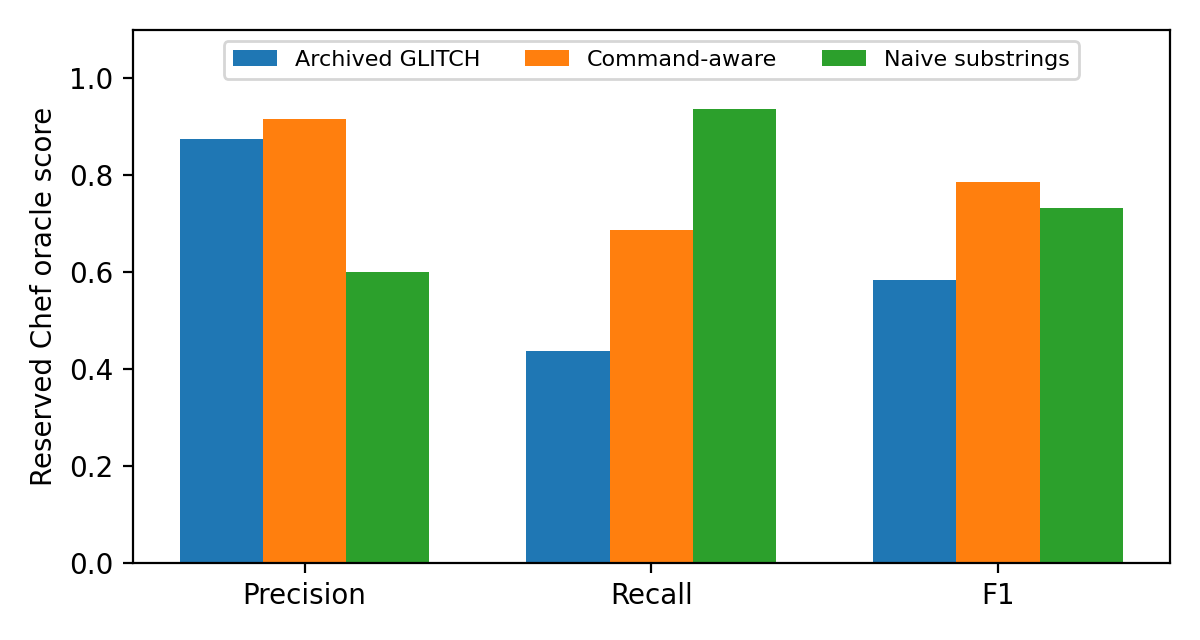
\includegraphics[width=\columnwidth]{chef_holdout.png}
\caption{Reserved Chef administrative-default results. The command-aware rule improves recall while retaining one false positive; naive substring matching adds false positives. These are point estimates on 16 annotated occurrences.}
\end{figure}

\subsection{Verification and Cost}
\VerificationDiscussion{}
No training, GPU, or paid cloud runtime is necessary. Timing refers to local static analysis, not execution of the infrastructure. Numerical results are counts from the preserved oracle, not generated examples or copied paper values.

\section{Discussion and Limitations}
An IR-level extension preserves the polyglot design: the same rule can process common variable/attribute nodes from several IaC technologies. Nevertheless, command syntax remains a language boundary within those values. The recognizer is deliberately bounded and is not a complete shell interpreter. It does not infer users from external files, runtime state, defaults, arbitrary wrappers, or resolved variable values.

The oracle is small and was partly selected using detector reports in the original study~\cite{glitch2022}; recall/precision therefore need not transfer to a representative production sample. A file-disjoint holdout prevents within-file leakage but not correlations between scripts from the same originating project. Majority-vote annotations measure agreement with a smell definition, not exploitability. Administrative access can be necessary in legitimate provisioning, so a report should prompt review rather than automatic privilege removal.

Original Ansible content matching and selected file-level exceptions can credit reports with imprecise locations. Exact-line sensitivity therefore accompanies the published protocol. Cached outputs are explicitly labeled; native parsing may be affected by platform and Ruby-version differences even when Python analyzer source is identical. Any such differences are retained rather than concealed. \SpecificLimitations{}

The base paper itself identifies command-embedded users as a limitation. Our correction should therefore be described as an implementation and measured extension of GLITCH's archived behavior, not a newly discovered universal vulnerability or unprecedented algorithm. Larger project-disjoint datasets, richer command representations, and human review of false positives are appropriate next steps.

\section{Conclusion}
\MeasuredConclusion{}
An artifact-first workflow enables precise comparison and a bounded correction without changing the benchmark to suit the implementation. The source, partitions, predictions, matching protocols, rule freeze, and audit artifacts support inspection and rerunning.

\section*{Reproducibility and Submission Note}
The code, evaluation instructions, predictions, scores, tests, and extension are available in the public repository:\\
\url{https://github.com/SimoneRodriguess/glitch-cloud-security}.
Original GLITCH and derived code retain GPL-3.0-compatible terms. One historical oracle sample containing a private key is excluded from public redistribution; the repository provides a verified restoration procedure for local evaluation. All results and institutional AI-assistance rules should be reviewed before submission. This is an IEEE conference-format student research report, not an accepted IEEE publication.

\bibliographystyle{IEEEtran}
\bibliography{references}
\end{document}
